\subsection*{Proposed architecture}
Similar to time-domain direct-form IIR filter design, which relies on feeding back the filter's recursive part with a combination of delayed instances of its output (see Figure \ref{fig:IIR_feedbachArch}), our approach relies on spatial feedback of received array signals back to the transmitter.
\begin{figure}[!h]
\begin{center}
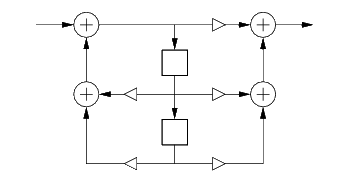
\includegraphics[width=0.5\linewidth]{./Media/BASIC_IIR_FILTER_ARCH.png}
\caption{Direct form IIR architecture. This architecture is based on feeding the input to the recursive part with delayed and weighted instances of its output.}
\label{fig:IIR_feedbachArch}
\end{center}
\end{figure}
In order to do so, we propose a dual beam-former architecture (see Figure \ref{fig:Proposed_spatialIIR_ARCH}), defined by two sets of spatial weights $\vecnot{\alpha},\vecnot{\beta}$, generating two independently spatially filtered signals $\vecnot{\alpha}^{T}\Steer{\theta_{g}},\vecnot{\beta}^{T}\Steer{\theta_{g}}$. One is the system's output and the other is fed back to the medium using a transmitting antenna.
\begin{figure}[!h]
\begin{center}
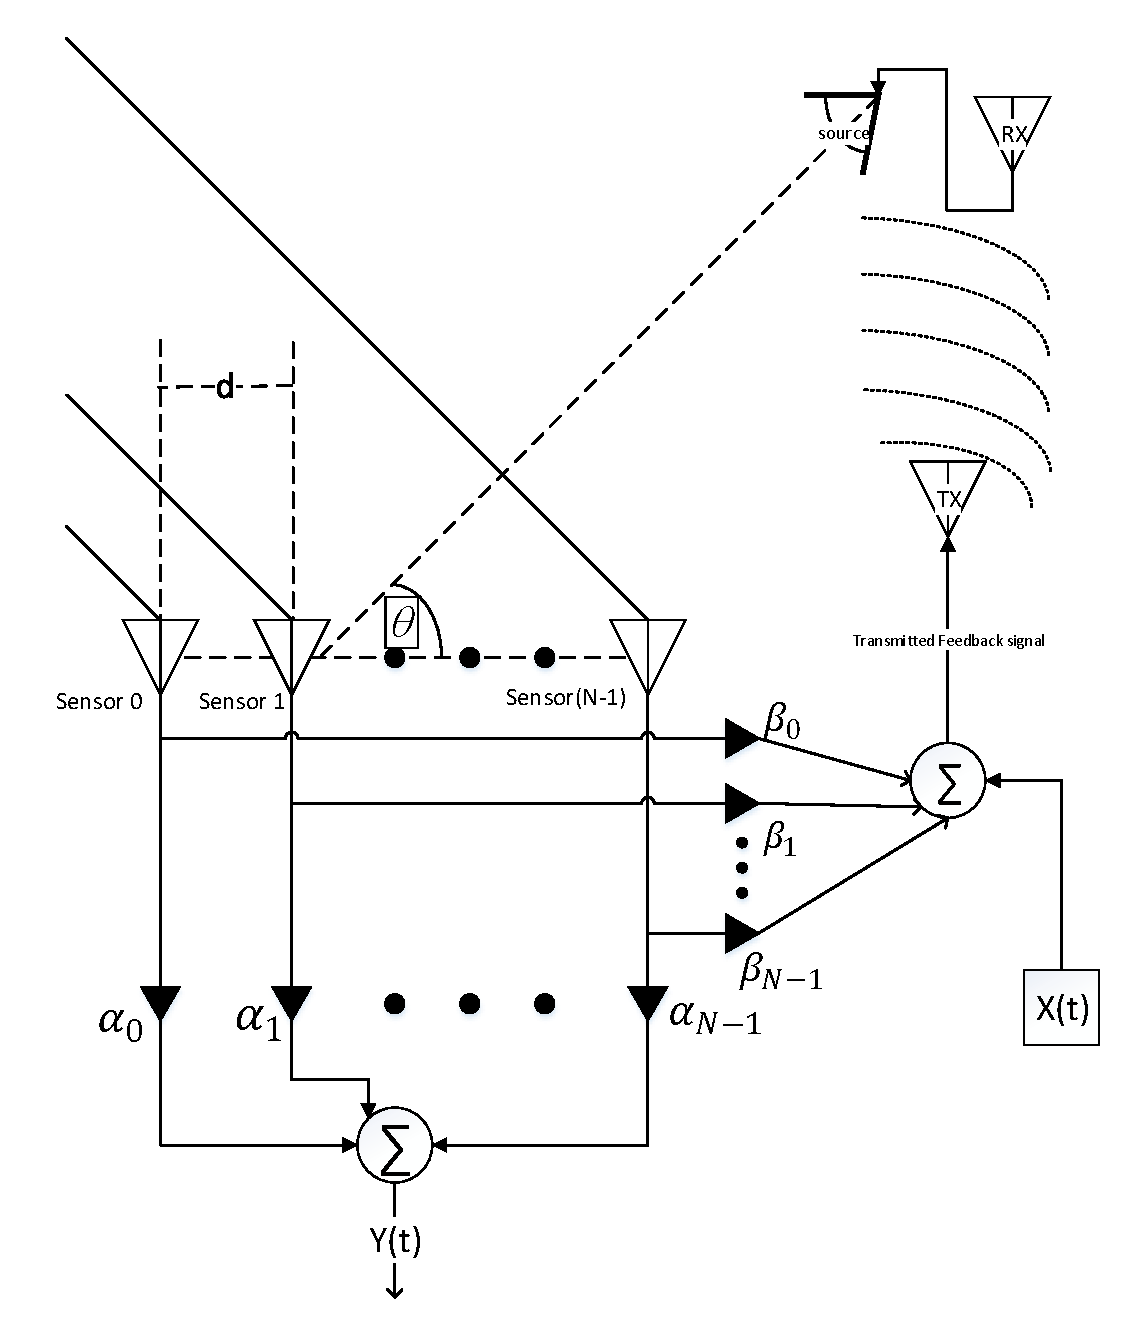
\includegraphics[width=0.75\linewidth]{./Media/SpatialIIR-diagram/SpatialIIR_VER5.pdf}
\caption{The proposed ``dual beam-former`` architecture. One beam-former, $\vecnot{\alpha}$, is generates the output signal. The other $\vecnot{\beta}$ synthesize the feedback transmission.}
\label{fig:Proposed_spatialIIR_ARCH}
\end{center}
\end{figure}
\subsection*{The proposed system's spatial response}
Time domain analysis of the proposed feedback based architecture, considering both propagation delay and attenuation, gives rise to
\begin{equation}
    \label{eqn:SingleSensorTemporalEquality}
    % \resizebox{.91\linewidth}{!}{
        \begin{split}
            x_{n}(t) = g\rBrace{s\rBrace{t-\tau_{pd}-\tau_{n}}
            +\sum_{m=0}^{N-1}{\alpha_{m}x_{m}\rBrace{t-\tau_{pd}-\tau_{n}}}},
        \end{split}
    % }
\end{equation}
where the first term of the right-hand side represents the contribution of the transmitted waveform $s(t)$ to the $n$'th array element and the second term represents the feedback contribution of the re-transmitted array signal to this same element.
Expressing \eqref{eqn:SingleSensorTemporalEquality}'s Fourier transform,
\begin{equation}
    \label{eqn_singleSensorFourier}
    % \resizebox{.91\linewidth}{!}{
        \begin{split}
            \F{x}_{n}\rBrace{\omega} =
            g\Bigg( & \F{s}\rBrace{\omega}
            \exp\rBrace{-j\omega\rBrace{\tau_{pd}+\tau_{n}}}
            \\&+\sum_{m=0}^{N-1}
            {
            \alpha_{m}\rBrace{\omega}\F{x}_{m}\rBrace{\omega}
            \exp\rBrace{-j\omega\rBrace{\tau_{pd}+\tau_{n}}}
            }\Bigg),
        \end{split}
    % }
\end{equation}
and its vector from,
$$
\F{\vx}\rBrace{\omega} = ge^{-j\omega\tau_{pd}} \rBrace{\F{s}\rBrace{\omega}+\vAlphaT \F{\vx}\rBrace{\omega}}\vd,
$$
we find that it can be simplified to
$$
\F{\vx}\rBrace{\omega} =\rBrace{I-g\vd\vAlphaT{}e^{-j\omega\tau_{pd}}}^{-1}g\vd\exp{\rBrace{-j\omega\tau_{pd}}}\F{s}\rBrace{\omega}.
$$
Then, denoting
\[
\phi\triangleq\omega\tau_{pd}
\]
as the round-trip signal propagation related electrical phase and using the Woodbury matrix identity \cite{woodbury1950inverting}, we find that
$$
\F{\vx}\rBrace{\omega}
=
\frac{    
g\vd\exp{\rBrace{-j\phi}}
}{
1 - g\aTd{}\exp{\rBrace{-j\phi}}
}\F{s}\rBrace{\omega}.
$$
Considering the noiseless case $\rBrace{\text{i.e. n}\rBrace{t}=0}$,
we express the general spatial response of FB as 
\begin{equation}
\label{eqn:GeneralFeedbackTransferFunction}
\Hba
\triangleq
\frac{\F{z}\rBrace{\omega}}{\F{s}\rBrace{\omega}} 
=
\frac{    
g\bTd{}\exp\rBrace{-j\phi}
}{
1 - g\aTd{}\exp\rBrace{-j\phi}
}.
\end{equation}
\par Note that this result confirms that our suggested array architecture achieves a controllable (via setting of $\vBeta$ and $\vAlpha$) and recursive (non-trivial denominator) spatial response.
As will be shown, high directivity and narrow beam-width are obtainable by proper selection of the weights. Comparing to traditional beamformers (i.e. with no feedback), the performance improvement will be expressed in terms of aperture increase, expressing the traditional beamformer aperture which achieves the same performance.
One may observe that opposed to traditional beamformers, the beampattern, $\Hba,$ is not only influenced by the impinging signal DOA, for it is also range selective due to its dependency on the phase parameter $\phi$.
As exemplified in Fig.~\ref{fig_rangeAzimuthSelectivity}, the combination of both angular and range selectivity enables the designer to enhance signals arriving from specific locations rather than only specific directions.
\begin{figure}[t!]
    \begin{center}
        \begin{overpic}[width=0.65\linewidth, 
        % grid, 
        tics=10,trim=0 0 0 0]{./Media/azimuthRangSelectivity.png}
            \put (20, 23){\rotatebox{0}{\footnotesize{Angular response}}}
            \put (30.5, 47){\rotatebox{0}{\footnotesize{Enhanced radial slice}}}
        \end{overpic}
    \end{center}
     \caption{A visualization of the spatial area selectivity concept. Combining both radial selectivity (i.e. enhancing signals from a specific distance) and DOA-based selectivity, allows the enhancement of signals arriving from specific areas (grey filled), while signals originated in other areas (even from the same DOA) are suppressed.}
    \label{fig_rangeAzimuthSelectivity}
\end{figure}
\section{Fisher information matrix}
A possible evaluation for the contribution of the presented feedback mechanism is to measure the additional information in the system.
To this end, the FIM will now be calculated with respect to the DOA parameter $\thetaD$ and the range related parameter $\phi$. 
As the feedback-based transfer function (\ref{eqn:GeneralFeedbackTransferFunction}) is expressed in the frequency domain, we rely on \cite{zeira1990frequency}, to express the FIM in the frequency domain as well. 
\par A single element of the FIM, notated by the matrix $J$, can be expressed as
\begin{equation}
    \resizebox{.9\linewidth}{!}{
        \begin{split}
            J_{\vBrace{k,l}}\rBrace{\vEta} 
            =&
            \Re\cBrace{
            \frac{1}{2\pi}
            \int_{-\omega_{s}/2}^{\omega_{s}/2}
            {
            \frac{1}{\Phi\rBrace{\omega}}
            \mathfrak{F}^{*}\left\{
            \frac{\partial z(t)}{\partial\eta_{k}}
            \right\}
            \mathfrak{F}\left\{
            \frac{\partial z(t)}{\partial\eta_{l}}
            \right\}
            d\omega
            }}
            \\ &+
            \frac{T}{4\pi}
            \int_{-\omega_{s}/2}^{\omega_{s}/2}
            \frac{1}{\Phi^{2}\rBrace{\omega}}
            \frac{\partial\Phi\rBrace{\omega}}{\partial\eta_{k}}
            \frac{\partial\Phi\rBrace{\omega}}{\partial\eta_{l}}
            d\omega
        \end{split}
    }
\end{equation}
where $ \vEta = [\thetaD,\phi]^{T} $ is the parameters vector, $\Re$ stands for the real-part extraction operator, $k,l \in\cBrace{1,2}$, $\Phi\rBrace{\omega}$ is the noise spectrum, $\mathfrak{F}$ is the Fourier transform operator, $T$ is the measurement observation interval and $\omega_{s}$ is the signal bandwidth. 
For simplicity, $\text{n}\rBrace{t}$ is assumed to be white and Gaussian with some constant power spectral density $\Phi(\omega)=\sigma^2$ and does not depend on the estimated parameters $\eta$, hence the second term vanishes. 
Assuming continuously differentiable functions, where order alteration of the Fourier transform and the differentiation operations is allowed, the FIM's $\vBrace{k,l}$'th element is
\begin{equation}
    \label{eq_beamPatternFreqDomain_FIM}
    % \resizebox{1\linewidth}{!}{
        \begin{split}
            J_{\vBrace{k,l}}\rBrace{\vEta} = 
            \Re\cBrace{
            \frac{1}{2\pi\sigma^2}
            \int_{-\omega_{s}/2}^{\omega_{s}/2}
            {
            \rBrace{\frac{\partial{}\F{z}\rBrace{\omega}}{\partial\eta_{k}}}^{\ast}
            \frac{\partial{}\F{z}\rBrace{\omega}}{\partial\eta_{l}}
            d\omega
            }}
        \end{split}.
    % }
\end{equation}
For omni-directional array sensors, $g$ is independent of the estimated parameters, therefore
\begin{equation}\label{eq_vdDiff}
\frac{\partial\vd}{\partial\thetaD}=A\rBrace{\omega}\vd
\end{equation}
where $A\rBrace{\omega}$ is an $N\times{}N$ diagonal matrix and each of its diagonal elements may expressed as 
\[
A_{\vBrace{i,i}}\rBrace{\omega}=-j\omega\frac{\partial \tau_{i}}{\partial{\thetaD}}\ \  \forall{i\in\cBrace{0\hdots{}N-1}}.
\]
To further simplify the analysis, without loss of generality, we use (in this section only) $g=1$.
In App.~\ref{apdx_clacFim} we compute the FIM terms, concluding that
\begin{equation}
    \label{eqn_FIMelements}
    \resizebox{.91\linewidth}{!}{
        \begin{split}
            &J_{\theta\theta}
            =
            \frac{1}{2\pi\sigma^{2}}\int_{-\omega_{s}/2}^{\omega_{s}/2}{\frac{
            \lBrace{\vBetaT{}A\rBrace{\omega}\vd-\vBetaT{}B\rBrace{\omega}\vAlpha\ePhi{-}}^{2}
            }{
            \lBrace{\rBrace{1-\aTd\ePhi{-}}^{2}}^{2}
            }\lBrace{\F{s}\rBrace{\omega}}^{2}d\omega}
            \\
            &J_{\phi\phi}
            =
            \frac{1}{2\pi\sigma^{2}}\int_{-\omega_{s}/2}^{\omega_{s}/2}{\frac{
            \lBrace{\bTd}^{2}
            }{
            \lBrace{\rBrace{1-\aTd\ePhi{-}}^{2}}^{2}
            }\lBrace{\F{s}\rBrace{\omega}}^{2}d\omega}
        \end{split}
    }
\end{equation}
where $B\rBrace{\omega}\triangleq\vd\vdT{}A\rBrace{\omega}-A\rBrace{\omega}\vd\vdT$.
Also, using some mild assumptions and setting
\begin{equation}\label{eq_alphaBetaPropSteer}
    \vAlpha,\vBeta\propto\vd^{\ast},
\end{equation}
we show that the cross terms of the FIM are nullified, i.e. $J_{\theta\phi} = J_{\phi\theta}^{*}=0$.
\par 
Choosing the weights as in \eqref{eq_alphaBetaPropSteer} may be interpreted as a generalization of the conventional beamformer (CB) \cite{van2004optimum}, more commonly referenced as the delay-and-sum (DS) beamformer which coherently integrate the impinging signal along the array elements.
The same choice of weights also minimizes the $\lBrace{1-\aTd\ePhi{-}}$ term, significantly increasing the available information, as predicted by the FIM.
It is worth mentioning that \eqref{eq_vdDiff} is relevant even for arbitrary (non-omni-directional) sensors when smooth and slowly changing radiation patterns are assumed.
In practice, though, there will be unavoidable errors, and perfect knowledge of the steering vector $\vd$ is not always available.
In Sec.~\ref{sec_Performance}, we quantify the effect of mismatching $\vAlpha$ with the desired form and discuss its influence on the array performance. 
\section{Performance of array processing with feedback}
In this section we analkyze some of the frundamental properties of an array; it's beamwidth and it's peak to a sidelobe level. As we show, by integrating the feedback, we can obtain performance much better than the classic  beamforming. We analyze the performance for general manifold, and then show the obtained results for a ULA. 
\subsection{Array beamwidth}
The Half-Power-Beam-Width (HPBW) parameter quantifies the array's main lobe narrowness, marking the DOA where the beampattern's energy reduces to half of its maximal value.
For standard ULA, with aperture of $N\delta$, it is known \cite{van2004optimum} that for large $N$,
$$
 \frac{\lambda\dThetaHPBW}{2\pi{}\delta} = \frac{\lambda}{\pi{}N\delta}1.4,
$$
where $\lambda$ is the signal wavelength and $\dThetaHPBW/2$ is the electrical angle where the HPBW is obtained. This result is more commonly expressed as $\dThetaHPBW/2= 1.4/N$. 
\par In App.~\ref{apdx_HPBW} we extend this known result for any $r\geq 0$. It turns out that for large $N$, the HPBW is obtained by solving the equation
\begin{equation}\label{eq_HPBW}
    % \resizebox{1\linewidth}{!}{
        \begin{split}
            \rBrace{r^{2}-4r+2}\frac{\sin{\rBrace{x}}^{2}}{x^{2}}+r\frac{\sin{\rBrace{2x}}}{x}-1=0
        \end{split}
    % }
\end{equation}
where we define $x\triangleq{} N\dTheta_{HPBW}/2$. In Fig.~\ref{fig_feedbackULA_HPBW_Nx_vs_N_variousR} we plot the numerical solution of \eqref{eq_HPBW} for various values of $r$ and $N$, showing that $x$ reaches its limit around $N=20$. Also note that for $r=0$ we obtain the known result of standard ULA with the limiting factor of $1.4$.
Having the limiting factors for various values of the gain mismatch $r$, we investigate the feedback related improvement, expressing the HPBW by
\[
\dThetaHPBW/2\approx \frac{1.4}{f(r)N}
\]
where $f(r)$ represents the array aperture improvement factor, compared to the standard ULA. 
Fig.~\ref{fig_feedbackULA_beamwidth_limit_r_dependent} shows that $f(r)$ is closely fitted with a second order polynomial
\begin{equation}
    \label{eq_Bapprox}
    f\rBrace{r}\approx\frac{1.4}{\rBrace{1-r}\rBrace{-0.4r+1.4}}.
\end{equation}
Note that for accurate gain match (i.e. $r\to1$), the right-hand-side of \eqref{eq_Bapprox} tends towards infinity, implying that the equivalent array has infinite number  of elements ($f\rBrace{r}N$), hence obtaining perfect spatial selectivity.
\begin{figure}[t]
    \begin{center}
        \begin{overpic}[width=0.65\linewidth, 
        %grid, 
        tics=10,trim=0 0 0 0]{./Media/spatial_IIR_MATLAB/arrayParameters/HPBW_vs_N_various_r.eps}
            \put (4, 75){\footnotesize{$N\dThetaHPBW/2$}}
            \put (50, 62.5) {\footnotesize{$r=0$}}
            \put (50, 54) {\footnotesize{$r=0.1$}}
            \put (50, 39.5) {\footnotesize{$r=0.3$}}
            \put (50, 28.5) {\footnotesize{$r=0.5$}}
            \put (50, 19.75) {\footnotesize{$r=0.7$}}
            \put (50, 12.5) {\footnotesize{$r=0.9$}}
            \put (50, 2) {\footnotesize{$N$}}
        \end{overpic}
    \end{center}
     \caption{Plot of $x=N\dThetaHPBW/2$ vs. $N$, for various $r$ values, obtained by numerically solving \eqref{eq_HPBW}.}
    \label{fig_feedbackULA_HPBW_Nx_vs_N_variousR}
\end{figure}
\begin{figure}[t]
    \begin{center}
        \begin{overpic}[width=0.65\linewidth, 
        % grid, 
        tics=10,trim=0 0 0 0]{./Media/HPBW_limit_vs_r.eps}
            \put (39.5, 63.5) {\scriptsize{Numerical solution of \eqref{eq_HPBW}}}
            \put (39.5, 58.25) {\scriptsize{Polynomial fitting \eqref{eq_Bapprox}}}
            \put (39.5, 52.5) {\footnotesize{$\log_{10}f\rBrace{r}$}}
            \put (85, 75) {\footnotesize{$\log_{10}f\rBrace{r}$}}
            \put (4, 75){\footnotesize{$N\dThetaHPBW/2$}}
            \put (50, 2) {\footnotesize{$r$}}
        \end{overpic}
    \end{center}
    \caption{Evaluation of $N\dThetaHPBW/2$ for $N=100$ and its approximation $1.4/f\rBrace{r}$  (marked by red diamonds). $f\rBrace{r}$ is also presented, in logarithmic scale (dotted curve).} 
    \label{fig_feedbackULA_beamwidth_limit_r_dependent}
\end{figure}
\subsection*{Phase alignment sensitivity}
Although (\ref{eqn_arrayPerformance_beamwidth_fullEpxr})'s high sensitivity (see (\ref{eqn_arrayPerformance_beamwidth_approx})) to $\dTheta$ expresses the desirable ``sharp`` spatial IIR beampattern, it's high sensitivity to $\dTau$, as will be demonstrated, states that only target which reside in a very impractically specific range (i.e. $\tau$) will be enhanced. To evaluate the necessary accuracy, we compare $\Hr{\theta}{\tau}{2}$ to $2$, while setting $\dTheta=0$ (i.e. perfectly steered array). It follows that $$\frac{r}{\left|1-\rho\right|^{2}}\dTau^{2} = 1,$$ i.e. only a very small range interval $\Delta{R} \triangleq \frac{\dTau}{2\pi{}\lambda}$ is amplified. Setting typical physical parameters (both in RF or acoustic environments) result in $\Delta{R} \propto 10^{-4}_{\left[m\right]}$ which is obviously impractical, considering array ambiguity, signal modeling errors, range estimation errors etc.